\section{Postscript: Reconsidering Divergence Cleaning in \arepo}
\label{sec:c4_postscript}

In Sec. \ref{sec:c4_discussion} we discussed why \arepo\ was capturing (at least some proxy of) rapid magnetic amplification during the merger when Eulerian simulations of NS mergers at similar resolutions cannot.  Since the publication of \citeal{zhu+15}, it has been pointed out that amplification could be the spurious result of \arepo's divergence cleaning mechanism.

%The MHD equations of motion (Eqn. \ref{eqn:c3_mhd_eqns}) do not contain $\bf{\nabla\cdot B}$, since they are identically zero according to Maxwell's Equations.

In most multidimensional numerical MHD schemes, the ``divergence constraint'' of $\bf{\nabla\cdot B} = 0$ is not guaranteed, and if the implicit divergence terms in Eqn. \ref{eqn:c3_mhd_eqns} are not considered, these schemes can in practice lead to spurious forces and magnetic instabilities \citep{toth00, hopkr16}.  A number of solutions exist (eg. \citealt{toth00}), and the most widely-used is \cite{evanh88}'s constrained transport (CT) method, which staggers the different components of the magnetic field within the discretization to keep the divergence constant in time to round-off errors (making it only necessary to initialize the simulation with $\bf{\nabla\cdot B} = 0$; see \citep{toth00}, Sec. 4.1).  This reliance on grid geometry, however, makes it challenging to implement in a moving mesh code (see \citealt{moczvh14} for recent work).  \arepo\ instead uses either the \cite{dedn+02} or \cite{powe+99} divergence control schemes.  The former introduces an additional conserved scalar term $\psi$ which is coupled to $\bf{\nabla\cdot B}$ while simultaneously being advected and forced to exponentially decay, while the latter adds source terms proportional to $\bf{\nabla\cdot B}$ that passively advects divergence errors, but does not damp them.  The Dedner method is superior because it actively minimizes divergence errors rather than simply preventing their local accumulation, but its implmentation in \arepo\ requires prohibitively small timesteps and tended to become unstable in highly dynamic environments \citep{pakms13}, hence our use of the Powell scheme, which can incur significant divergence errors.

% DEFENSE NOTEL: if the implicit divergence terms in Eqn. \ref{eqn:c3_mhd_eqns} are not considered, these schemes can in practice lead to spurious forces and magnetic instabilities that do not become negligible even at infinite resolution

% DEFENSE NOTE: Pakmor+11 uses the GLM-MHD method, though I find Eqn. 10 of Hopkins and Eqn. 24 of Dedner+02 to be the cleanest representations of this method.  Note that \psi is not proportional to B, but rather just coupled to it - see Eqn. 5 of Dedner, and the explanation around Eqn. 18, which shows that \psi in general has parabolic and hyperbolic (exponentially decreasing) components, leading to both exponential damping as well as transport via waves.

\begin{figure}
\centering
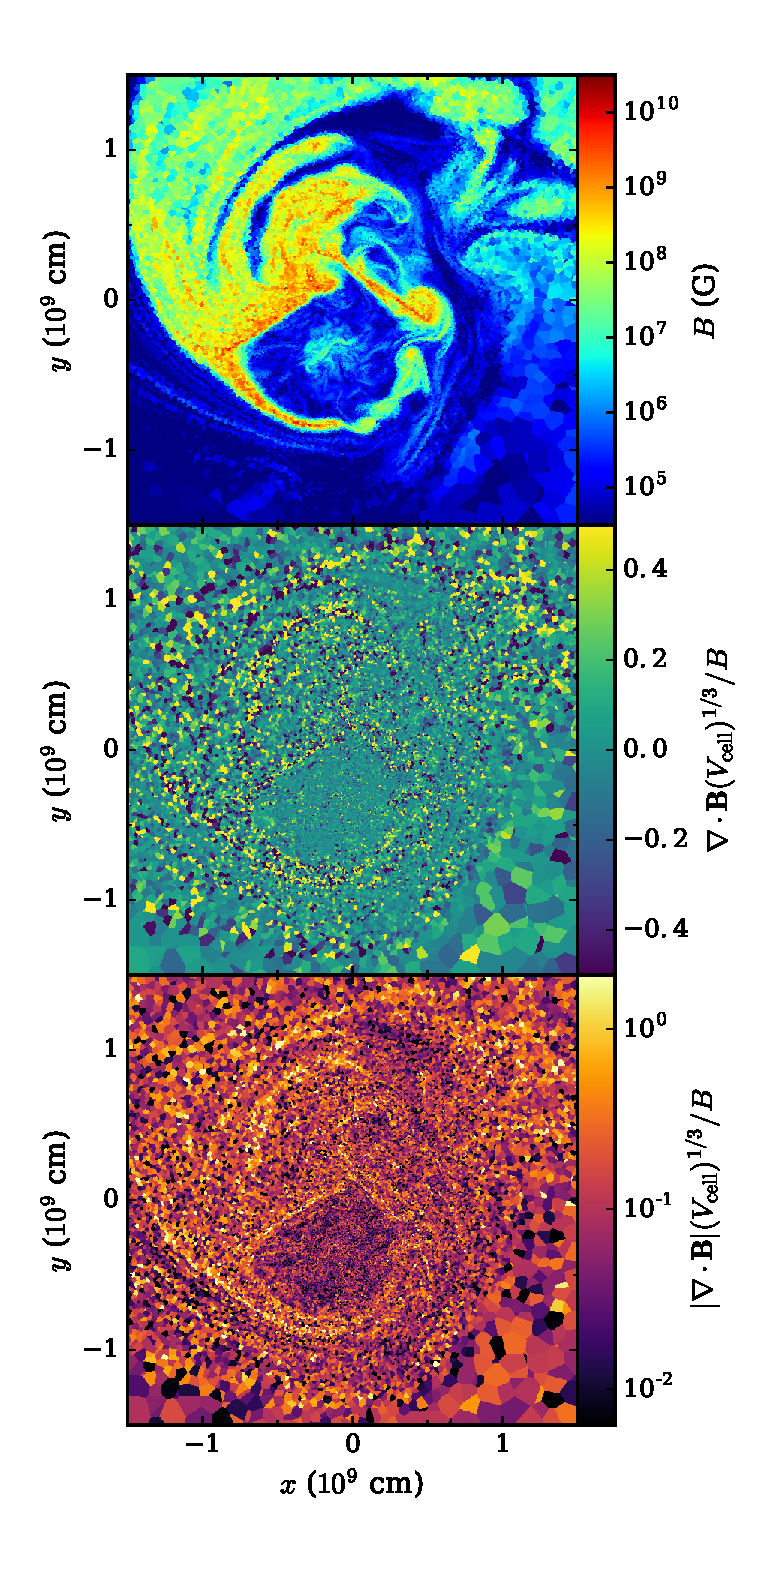
\includegraphics[angle=0,width=0.6\columnwidth]{chapter4_zhu+15/figures/bdiv.pdf}
\caption{From top to bottom, equatorial plane intensity profiles for the magnetic field strength, relative divergence error (linear scale) and absolute relative divergence error (logarithmic) for the simulation at $200\,\mrm{s}$.}
\label{fig:c4_bdiv}
\end{figure}

In Fig. \ref{fig:c4_bdiv} we plot the magnetic field strength, relative divergence error and absolute relative divergence error of our fiducial merger simulation at $t = 200\,\mrm{s}$, when the donor has just been disrupted.  The (mass-weighted) average relative divergence error $\left\langle|\mathbf{\nabla\cdot B}|(V_\mrm{cell})^{1/3}/B\right\rangle = 0.18$, where $V$ is the Voronoi cell volume, is typical of both this simulation and \citep{pakms13}'s, but much larger than typical results from Dedner cleaning-based codes \citep{tric15, hopkr16}.  As in \cite{pakms13}'s galaxy disk evolution simulation, the divergence error alternates on very small scales (Fig. \ref{fig:c4_bdiv} middle panel), and peaks near large magnetic gradients (comparing top and bottom panels).  While divergence errors cancel over larger scales (the average relative error with the sign of the divergence included, $\left\langle\mathbf{\nabla\cdot B}(V_\mrm{cell})^{1/3}/B\right\rangle = -1.4\times10^{-3}$), the regions of highest magnetic gradient correspond to the shear interface between donor and accretor, where we believe the field is amplified.  It is therefore plausible that, even though divergence errors cancel out over large scales, divergence errors at small scales spuriously magnify the magnetic dynamo associated with the shear layer and Kelvin-Helmholtz vortices.  

This hypothesis is supported by \cite{hopkr16}, who perform a battery of tests comparing the Dedner and Powell mechanisms for their mesh-free finite-volume code \textsc{GIZMO}, and show divergence errors in Powell-based simulations of advection and hydromagnetic instability and turbulence lead to unstable spurious field growth.  At the same time, however, \cite{pakmbs11} and \cite{pakms13} find good agreement between CT-based Eulerian simulations and Dedner and Powell-based \arepo\ simulations of the Orzag-Tang vortex problem\footnote{\cite{hopkr16} note that the Orzag-Tang vortex is one test problem where their Powell-based simulation returns results similar to their Dedner-based ones, and so the problem may not be generally representative of differences between the two.}, and the field growth rate in a simulation of the magneto-rotational instability is comparable to its analytic value, as well as to CT-based grid codes \citep{floc+10}.  The evidence that the Powell scheme produces spurious field amplifications in our simulations is thus quite concerning, but inconclusive.

%In Hopkins's most extreme test, SPH returns divergence errors of order 0.1 - 1 (Gizmo 0.01 - 0.1), but Arepo (pakmor+13) gives errors of order unity!

Caution is therefore in order when using this chapter's results, and further testing of \arepo's MHD scheme for stellar mergers is needed.  One possibility is to test-run mergers in \arepo\ using the Dedner method, as well as CT further in the future, which would allow us to compare simulations whose only difference is the divergence cleaning method.  A simpler test case would be simulations of field evolution within a single Kelvin-Helholtz vortex at various resolutions compared to the results of \cite{oberam10} and \cite{zrakm13}, both of which use Eulerian codes with CT.  Meanwhile, the remnant magnetic field's bulk properties following coalescence are physically plausible, as discussed in Sec. \ref{sec:c4_results}, and from above are likely to be more robust than the detailed field configuration.  We cite these properties (alongside \cite{ji+13}'s work) when considering magnetic simmering WDs the next chapter.

%\cite{pakmv13} find qualitative differences in their resolution test, which they attribute to large divergence errors artificially accelerating magnetic field growth in their low resolution simulations.  While we find no substantial difference in our test, we also check the divergence errors of our two simulations.  We find the time-averaged $\left\langle(\mrm{div} \vec{B}) r/B\right\rangle$ ($\left\langle|\mrm{div} \vec{B}| r/B\right\rangle$ during coalescence only) to be $1.1\times10^{-4}$ ($1.3\times10^{-1}$) for the fiducial run, and $2.0\times10^{-4}$ ($1.4\times10^{-1}$) for the low resolution run.  These errors are comparable to each other, and much smaller than any reported in \cite{pakmv13}.  Divergence errors are spatially highly localized and trace steep magnetic gradients, suggesting that these errors contribute only to small-scale variations in the magnetic field.  \textbf{Editors: $\left\langle(\mrm{div} \vec{B}) r/B\right\rangle$ begins at an enormous $10^{12}$; Ruediger, why would this be?  Did you see something similar in your simulations?}


